\documentclass[tikz,border=2pt]{standalone}
\usepackage{amsmath,amssymb,bm}
\usepackage[scaled=0.92]{helvet}
\usetikzlibrary{arrows.meta,positioning,fit,calc,backgrounds}

% same palette as the RSMA figure
\definecolor{cfill}{HTML}{DCE6F4}
\definecolor{cedge}{HTML}{2F4A73}
\definecolor{pfill}{HTML}{EEEEEE}
\definecolor{pedge}{HTML}{4D4D4D}
\definecolor{scol}{HTML}{7A3E8E}
\definecolor{grp}{HTML}{8C8C8C}
\definecolor{txfill}{HTML}{F4F6FA}
\definecolor{rxfill}{HTML}{F7F5F0}

\begin{document}
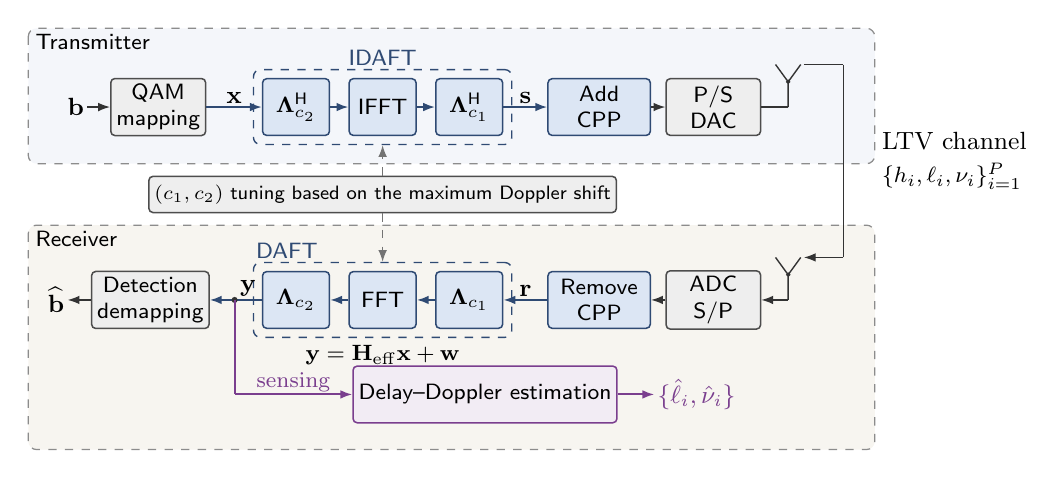
\begin{tikzpicture}[
    font=\small,
    >={Latex[length=1.5mm,width=1.1mm]},
    line/.style={draw=black!80, line width=0.5pt},
    cline/.style={draw=cedge, line width=0.7pt},
    sline/.style={draw=scol, line width=0.7pt},
    ctrl/.style={draw=black!55, line width=0.45pt, dashed},
    blk/.style={draw=pedge, line width=0.55pt, fill=pfill, rounded corners=1.5pt,
                minimum height=7.2mm, inner sep=2pt, font=\sffamily\footnotesize, align=center},
    cblk/.style={blk, draw=cedge, fill=cfill},
    mblk/.style={cblk, minimum width=8.5mm},
    sblk/.style={blk, draw=scol, fill=scol!10},
    lab/.style={font=\fontsize{9.2}{11}\selectfont, inner sep=1pt},
    sm/.style={font=\fontsize{8}{10}\selectfont, inner sep=0.8pt},
    grpbox/.style={draw=grp, dashed, line width=0.45pt, rounded corners=3pt, inner sep=4pt},
    opbox/.style={draw=cedge, dashed, line width=0.5pt, rounded corners=2.5pt, inner sep=3pt},
    grplab/.style={font=\sffamily\footnotesize, text=black, inner sep=1pt},
    dot/.style={circle, fill=black!80, inner sep=0pt, minimum size=2.2pt},
]

% ================= rows / columns =================
\def\yT{0}       % transmitter chain
\def\yR{-2.45}   % receiver chain
\def\yS{-3.65}   % sensing branch
\def\xL{-0.6}
\def\xR{10.15}
\def\xa{2.8}     % first chirp/FFT block
\def\xb{3.9}     % (I)FFT
\def\xc{5.0}     % second chirp block

% ---------- background panels ----------
\begin{scope}[on background layer]
  \draw[grpbox, fill=txfill] (\xL,1.0) rectangle (\xR,-0.72);
  \draw[grpbox, fill=rxfill] (\xL,-1.5) rectangle (\xR,-4.35);
\end{scope}
\node[grplab, anchor=north west] at (\xL+0.05,0.97) {Transmitter};
\node[grplab, anchor=north west] at (\xL+0.05,-1.53) {Receiver};

% ================= transmitter =================
\node[lab, anchor=east] (bits) at (0.15,\yT) {$\mathbf b$};
\node[blk, minimum width=12mm] (qam) at (1.05,\yT) {QAM\\mapping};
\node[mblk] (lc2h) at (\xa,\yT) {$\bm\Lambda_{c_2}^{\mathsf H}$};
\node[mblk] (ifft) at (\xb,\yT) {IFFT};
\node[mblk] (lc1h) at (\xc,\yT) {$\bm\Lambda_{c_1}^{\mathsf H}$};
\node[opbox, fit=(lc2h)(lc1h)] (idaft) {};
\node[grplab, text=cedge, above=0pt of idaft] {IDAFT};
\node[cblk, minimum width=13mm] (cpp) at (6.65,\yT) {Add\\CPP};
\node[blk, minimum width=12mm] (dac) at (8.1,\yT) {P/S\\DAC};

\draw[line,->] (bits) -- (qam);
\draw[cline,->] (qam) -- node[lab, above] {$\mathbf x$} (lc2h);
\draw[cline,->] (lc2h) -- (ifft);
\draw[cline,->] (ifft) -- (lc1h);
\draw[cline,->] (lc1h) -- node[lab, above] {$\mathbf s$} (cpp);
\draw[line,->] (cpp) -- (dac);

% tx antenna
\coordinate (txa) at (9.05,\yT);
\draw[line] (dac.east) -- (txa);
\draw[line] (txa) -- ++(0,0.32) -- ++(-0.16,0.22) ++(0.16,-0.22) -- ++(0.16,0.22)
  ($(txa)+(0,0.32)$) circle (0.5pt);   % one path = antenna symbol

% ================= channel =================
\coordinate (rxa) at (9.05,\yR);
\coordinate (ch1) at (9.75,{\yT+0.54});
\coordinate (ch2) at (9.75,{\yR+0.54});
\draw[line] ($(txa)+(0.2,0.54)$) -- (ch1);
\draw[line] (ch1) -- (ch2);
\draw[line,->] (ch2) -- ($(rxa)+(0.2,0.54)$);
\node[lab, anchor=west, align=left] at (10.2,{(\yT+\yR)/2+0.54})
  {LTV channel\\[1pt]\footnotesize $\{h_i,\ell_i,\nu_i\}_{i=1}^{P}$};

% ================= receiver =================
\draw[line] (rxa) -- ++(0,0.32) -- ++(-0.16,0.22) ++(0.16,-0.22) -- ++(0.16,0.22)
  ($(rxa)+(0,0.32)$) circle (0.5pt);   % one path = antenna symbol

\node[blk, minimum width=12mm] (adc) at (8.1,\yR) {ADC\\S/P};
\node[cblk, minimum width=13mm] (rcpp) at (6.65,\yR) {Remove\\CPP};
\node[mblk] (lc1) at (\xc,\yR) {$\bm\Lambda_{c_1}$};
\node[mblk] (fft) at (\xb,\yR) {FFT};
\node[mblk] (lc2) at (\xa,\yR) {$\bm\Lambda_{c_2}$};
\node[opbox, fit=(lc2)(lc1)] (daft) {};
\node[grplab, text=cedge, anchor=south west] at (daft.north west) {DAFT};
\node[blk, minimum width=12mm] (det) at (0.95,\yR) {Detection\\demapping};
\node[lab, anchor=east] (bhat) at (-0.1,\yR) {$\widehat{\mathbf b}$};

\draw[line,->] (rxa) -- (adc);
\draw[line,->] (adc) -- (rcpp);
\draw[cline,->] (rcpp) -- node[lab, above] {$\mathbf r$} (lc1);
\draw[cline,->] (lc1) -- (fft);
\draw[cline,->] (fft) -- (lc2);
\coordinate (yj) at (2.02,\yR);
\draw[cline] (lc2) -- (yj);
\draw[cline,->] (yj) -- (det);
\node[lab, above] at ($(lc2.west)!0.5!(yj)$) {$\mathbf y$};
\draw[line,->] (det) -- (bhat);
\node[dot] at (yj) {};

% effective channel annotation
\node[sm, below=1.5pt of daft] {$\mathbf y=\mathbf H_{\mathrm{eff}}\mathbf x+\mathbf w$};

% ================= chirp-parameter tuning =================
\node[blk, minimum height=4.6mm, minimum width=58mm, font=\sffamily\scriptsize] (tune) at (\xb,-1.11)
  {$(c_1,c_2)$ tuning based on the maximum Doppler shift};
\draw[ctrl,->] (tune.north -| idaft.south) ++(0,0) -- (idaft.south);
\draw[ctrl,->] (tune.south -| daft.north) -- (daft.north);

% ================= sensing branch (ISAC) =================
\node[sblk, minimum width=30mm] (sens) at (5.2,\yS) {Delay--Doppler estimation};
\coordinate (sj) at (2.02,\yS);
\draw[sline] (yj) -- (sj);
\draw[sline,->] (sj) -- (sens);
\node[lab, anchor=west, text=scol] (est) at (7.35,\yS) {$\{\hat\ell_i,\hat\nu_i\}$};
\draw[sline,->] (sens) -- (est);
\node[sm, text=scol, above] at ($(sj)!0.5!(sens.west)$) {sensing};

\end{tikzpicture}
\end{document}
